%----------------------------------------------------------------------------------------
% SECTION 1
%----------------------------------------------------------------------------------------
\section{Qualitative elemental identification of bilayer systems}
\subsection{Elemental identification}
% model performance
The model performance for the qualitative elemental identification is shown in Table \ref{tab:acc_qual}. The categorical accuracies were computed for the training on the mixcont dataset. 
During the model development, it was obvious that we are prone to overfitting the simulated data resulting in poor performance on test data. Especially, because we do not represent the experimental spectra with enough accuracy, we must make sure to focus on the robustness of the model. Thus, the obvious approach was to choose the most simple model which was able to train effectively without overfitting and before aiming at the highest accuracy rates. The models remained unchanged for the qualitative identification for all datasets. Thus, a total of 8 models were developed for task 1 - one of each model type for each layer and the models were trained on the three datasets. For each best performing model for each layer and dataset, the confusion matrices are shown.

\begin{table}[H]
    \centering
    \centerline{
    \begin{tabular}{c|c|c|c|c|c}
         Layer & Model   & No. Parameters & Training set & Validation set & Test set*    \\
        \hline 
        top   & CNN     &  8.2 M        &    92.37      &    \textbf{86.68} & 27.91       \\
              & CNN-DCT &  12.3 M        &   91.34        &    86.58       & 14.42           \\
              & CBAM    &  20.1 M        &  \textbf{92.80}       &    82.80       & 28.64          \\
              & ViT     &  35.8 K        &    79.92     &    82.69       & \textbf{52.56}  \\
        \hdashline
         bot   & CNN     &   8.2 M       &\textbf{89.05}&   \textbf{79.64}    &     45.12      \\
               & CNN-DCT &   12.3 M       &    85.39      &    79.39       &   50.23       \\
               & CBAM    &   20.1 M        &    86.65     &    70.96     &       27.44    \\
               & ViT     &   35.8 K      &     61.65     &      68.35    &  \textbf{57.21} \\
    \end{tabular}}
    \caption{Categorical accuracies, and number of parameters of the models in respect to dataset and sample layer
    *Test Dataset n=\nelementalspectra}
    \label{tab:acc_qual}
\end{table}


\subsubsection{Top layer prediction}
The best model to predict the top layer element was the Vision Transformer-Model, with an accuracy on the test dataset of 52.56 \%. Figure \ref{fig:top_best_loss} shows the categorical crossentropy loss and categorical accuracy for the training (blue) and the validation (orange) datasets respectively. In the confusion matrix, we can see that in the test dataset, Iron (Fe) has been wrongly predicted as Lithium (Li) a total of 4 times, which are the most failures of any wrongly predicted elements. An approach would be to plot the attention of the model on Lithium and Iron spectrum data to investigate the reason behind. However, as shown in Figures \ref{att:Fe} and \ref{att:Li}, they overlap at a binding energy of 55 eV. This is a known overlap of the Li 1s and Fe 3p peaks. However, as the attention does not focus on this part for the Iron spectrum, it is not obvious why this faulty prediction was done. It suggests that the model lacks complexity as both cases overlap in the feature space. As the model only has 25.8k trainable parameters, this is very much possible. 


\begin{figure}
    \centering
    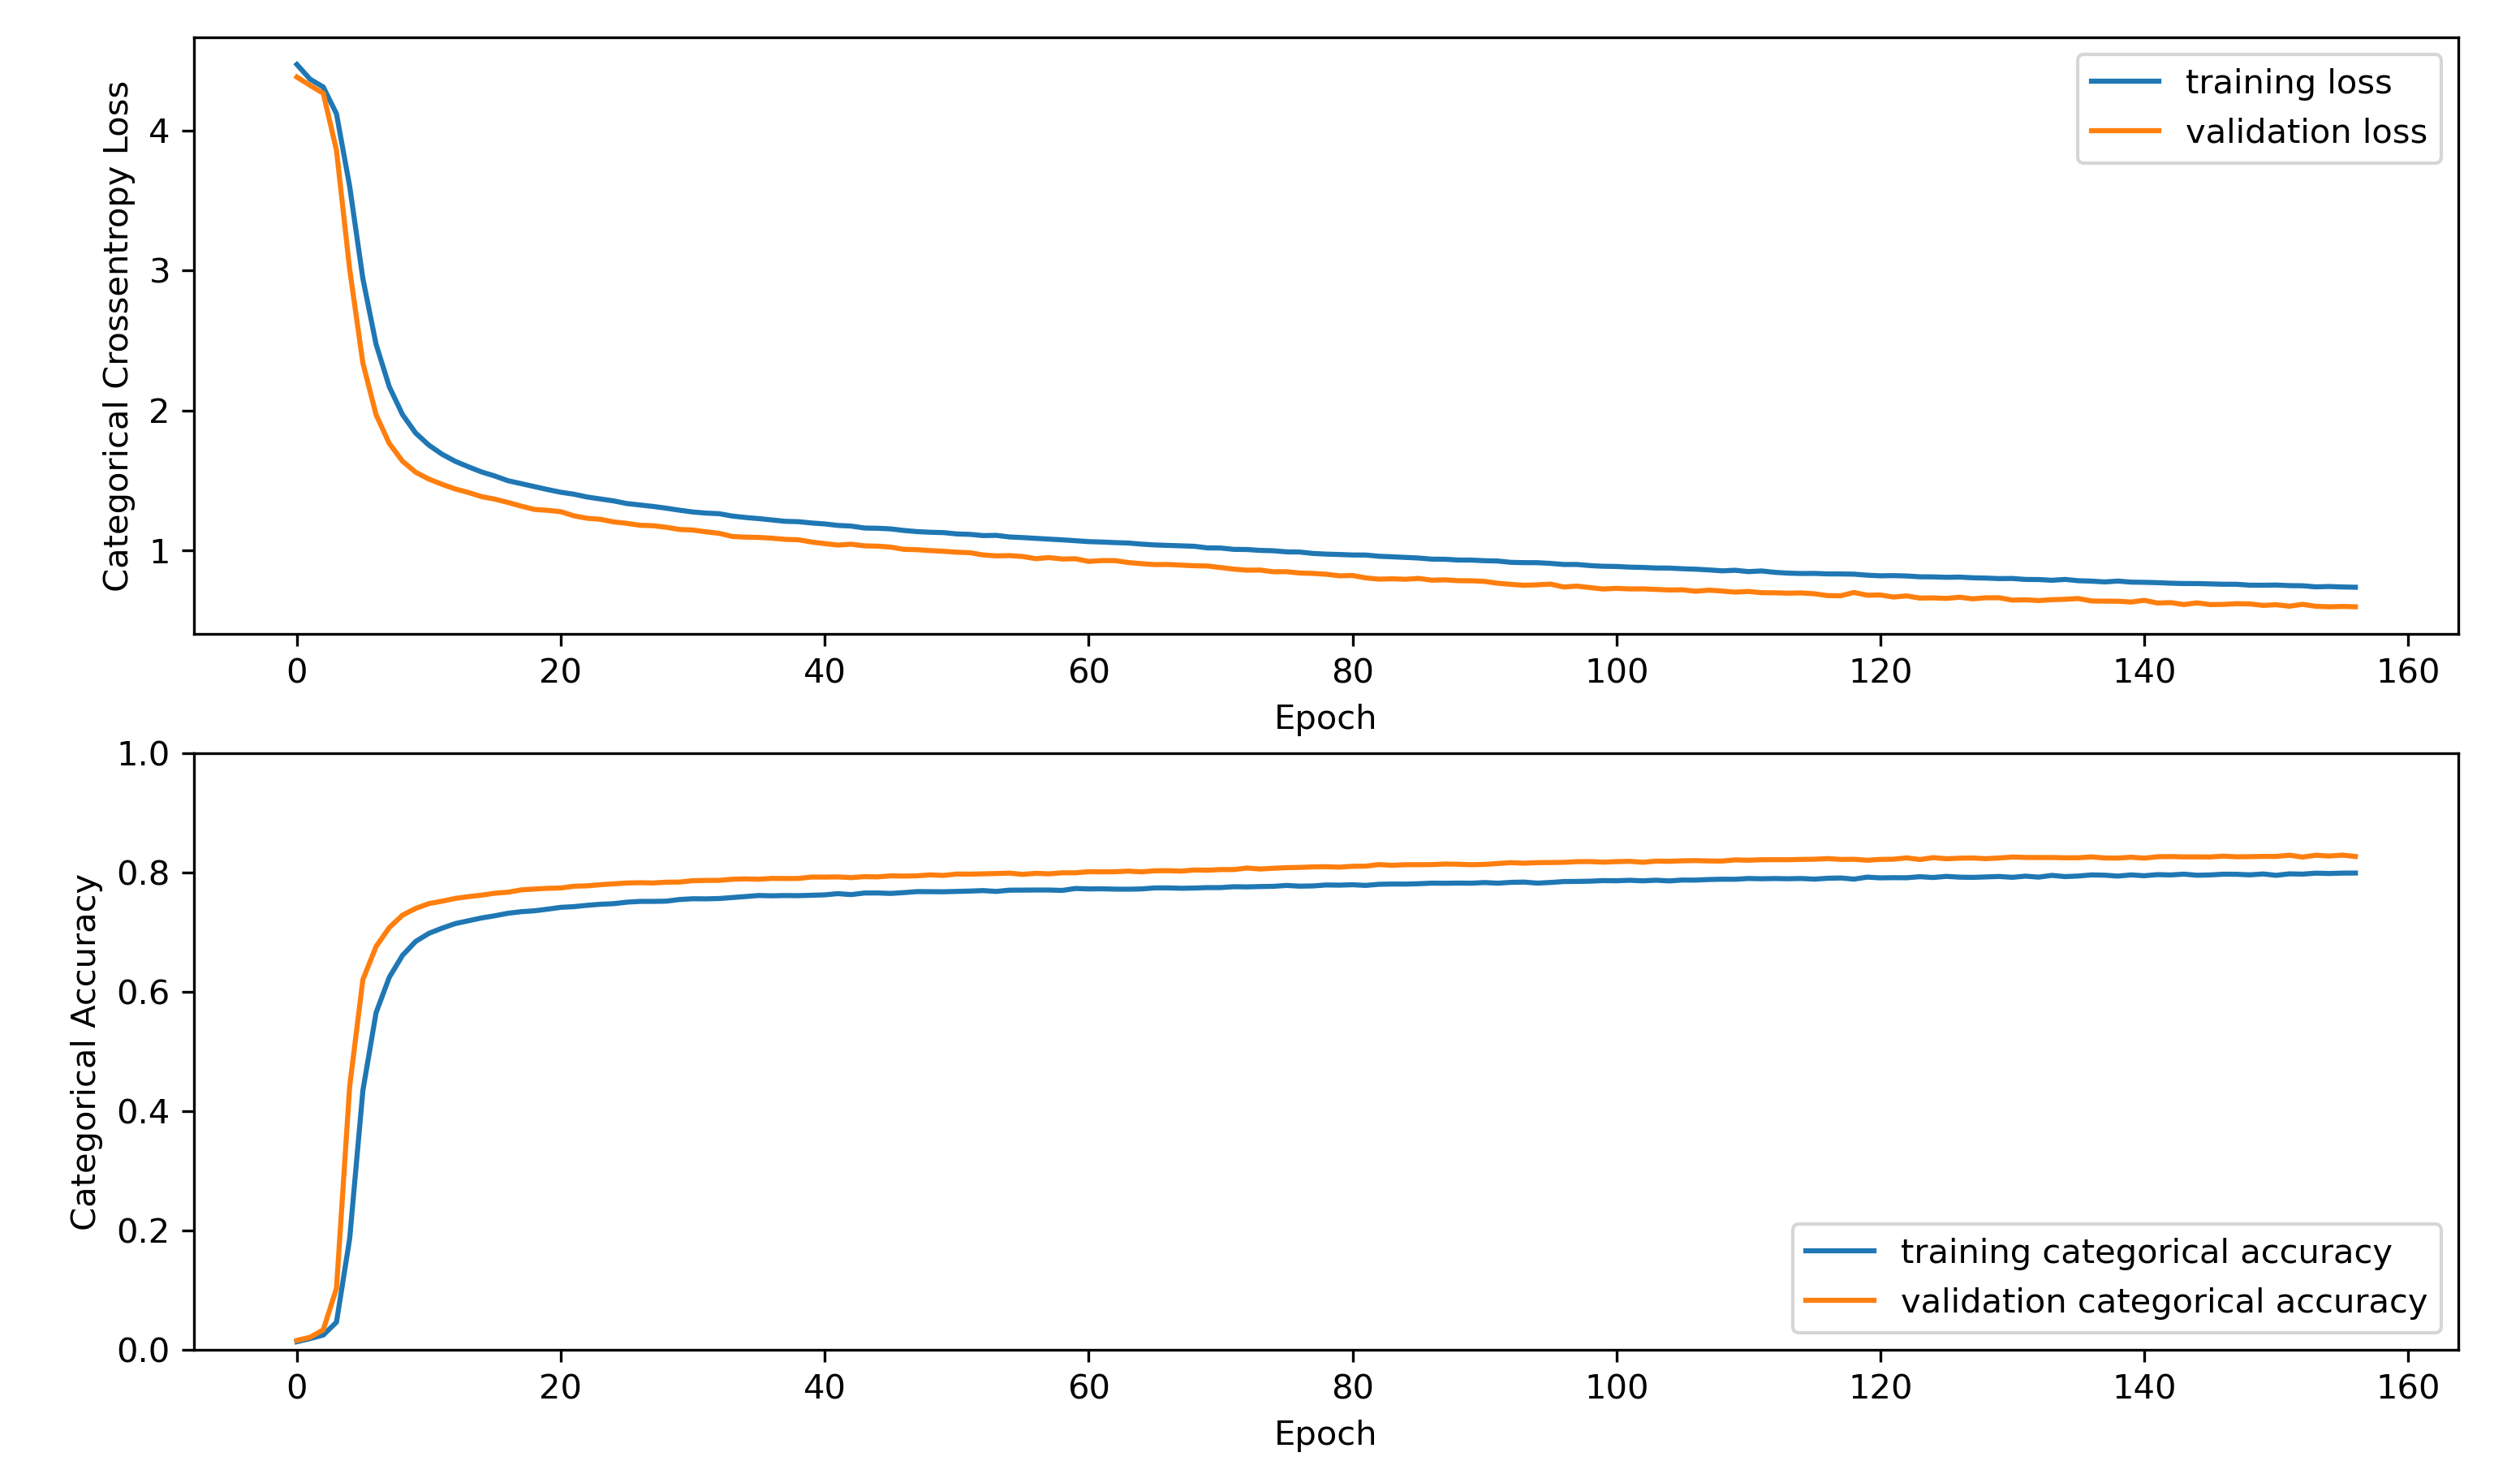
\includegraphics[width=0.7\textwidth]{Figures/best_task_1_model_loss.png}
    \caption{Categorical crossentropy loss and crossentropy accuracy for the ViT model training on top-layer training data-labels}
    \label{fig:top_best_loss}
\end{figure}

\begin{figure}[H]

    \begin{subfigure}[b]{1\textwidth}
            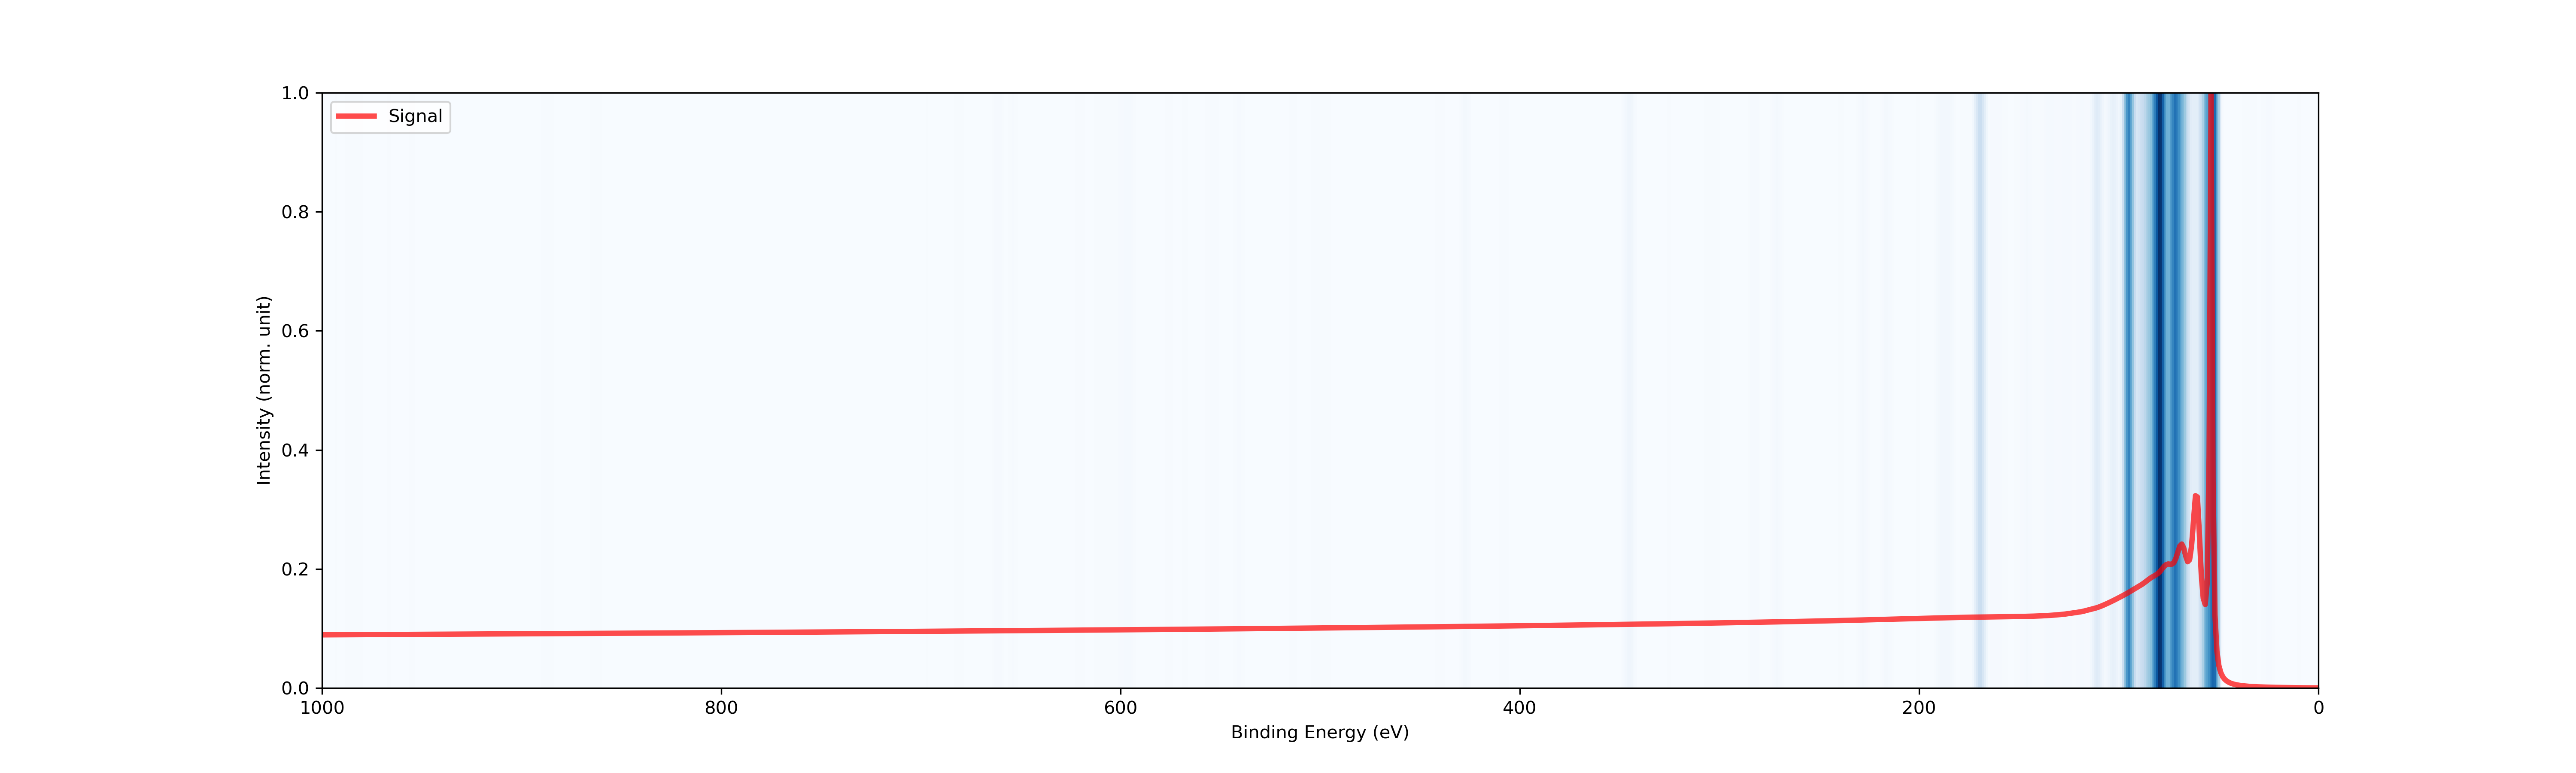
\includegraphics[width=\textwidth]{Figures/attention_map_Li.png}
            \caption{Attention map (blue) for the Lithium spectrum (red) prediction}
            \label{att:Li}
    \end{subfigure}
    \begin{subfigure}[b]{1\textwidth}
            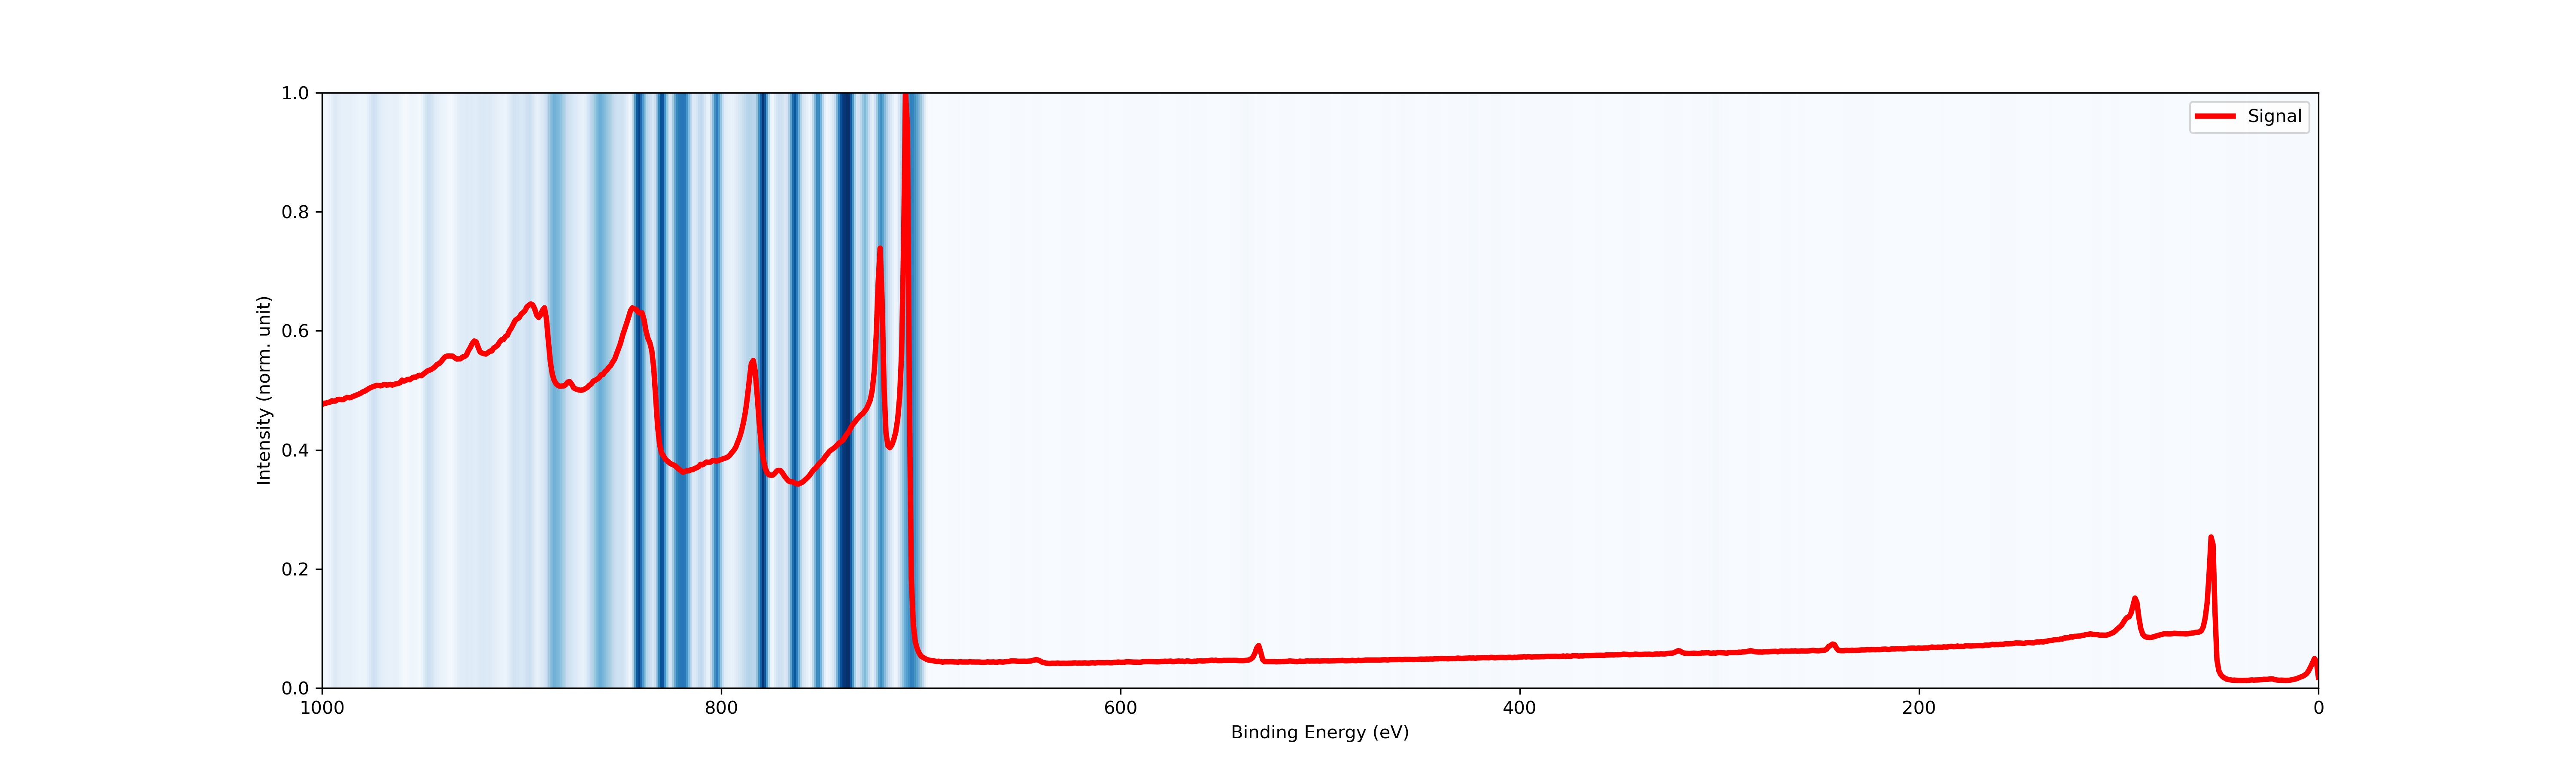
\includegraphics[width=\textwidth]{Figures/attention_map_Fe.png}
            \caption{Attention map (blue) for the experimental Iron spectrum (red) prediction}
            \label{att:Fe}
    \end{subfigure}
    
    \begin{subfigure}[b]{1\textwidth}
            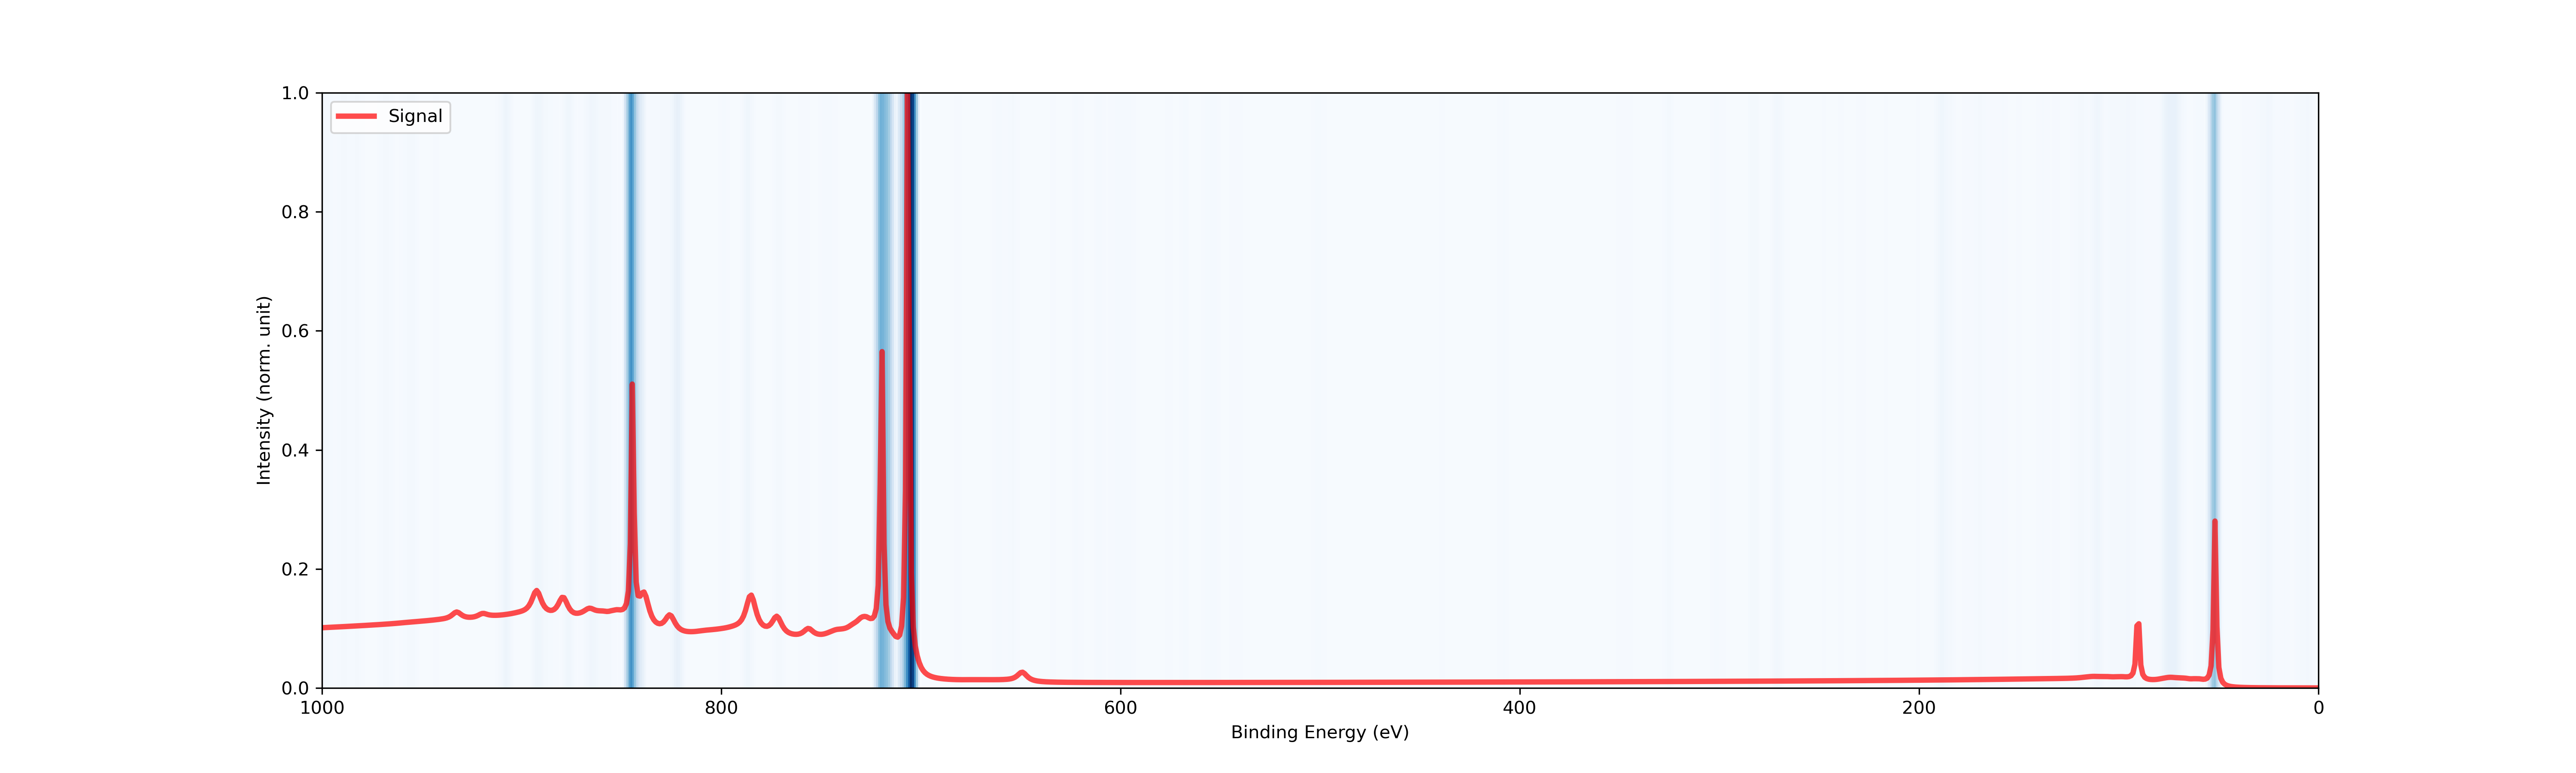
\includegraphics[width=\textwidth]{Figures/attention_map_Fe_Training.png}
            \caption{Attention map (blue) for the simulated Iron spectrum (red) prediction}
            \label{att:FeSim}
    \end{subfigure}
\caption{Attention maps of false top layer predictions}
\end{figure}


\begin{center}
\begin{figure}[H]
        \centerline{\includegraphics[width=1.4\textwidth]{Figures/best_task_1_model_CM.png}}
    \centering
    \caption[width=1.4\textwidth]{Confusion natrix of test dataset for best top-layer prediction}
    \label{cm_cnn_1l}
\end{figure}
\end{center}



\subsubsection{Bottom layer prediction}


From the experimental data, the same test dataset was used as for the top-layer prediction. Because survey scans of buried layers are rare, we considered pure elemental spectra to be composed of a buried layer of the pure element respectively.
From Table \ref{tab:acc_qual}, we can see that the performance of the bottom layer prediction is not always lower than the top layer prediction. However, we would expect a lower accuracy for the bottom layer, due to the principle of XPS measurement, as electrons from the deeper layer must travel through the top layer and thus will be less intense and more influenced by scattering from interactions. Anyway, as we consider experimental data from pure elements as a two-layer system in our test-set, it could also be that the simulated spectra from buried pure elements actually resembles ground truth more accurately. However, the most probable explanation is that the early stopping stopped the model from overfitting because it was harder to train the bot-layer labels due to the previously mentioned scattering effects.




\subsection{Depth profile determination of native oxides and elements}

% As there's almost no test data this is experimental
Depth profiling or determination of overlayer thickness is often conducted in scientific experiments. However, data is usually not publicly available - and if - it does often not include survey spectra. This is because these measures are usually done with ion-sputtering profiling or angle-resolved measurements and as these experiments are time-consuming, only the regions of interests (where the peaks are expected depending on the sample) are scanned.
As depth profiling data is not readily available from public databases, the datasets obtained internally as explained in chapter \ref{exp_depth}, were used to evaluate the model on experimental data. The models previously explained were slightly adapted for this task to train efficiently. For example, the CBAM model had a filter-size of 1024.

\begin{table}[H]
    \centering
    \begin{tabular}{c|c|c|c|c}
        Dataset & Model   & No. Parameters & Training set    & Validation set    \\
        \hline
 mixcont+oxides& CNN     &   8.2 M       &      50.75      &          42.66         \\
               & CNN-DCT &   12.2 M       &     38.06           &      37.24           \\
               & CBAM    &   40.1 M       &    46.65             &      39.19            \\
               & ViT     &    35.6 M     &      39.03            &       31.24           \\

    \end{tabular}
    \caption{Accuracies and number of parameters of the models for layer thickness prediction}
    \label{tab:acc_depth}
\end{table}

The test data contained seven spectra with the structure explained in \ref{exp_depth}. Each spectrum is evaluated with each model and the results are shown in Table \ref{tab:acc_depth}, where the Al-Oxide denotes the sample b) shown in Figure \ref{fig:exp_samples} and the Cu/Pd denotes the sample a). From the results, it is obvious that we are far from a good prediction model. However, we can interpret whether tendencies are correct. For the covered (2 and 1.5nm) Aluminum-Oxides, the prediction had the correct tendency for all models but the ViT-model. However, the predictions for the copper and palladium sample showed much less difference. It should be noted, that the 20 nm overlayer would never be predicted correctly with our model, because we did not include such data. However, by using the qualitative model for top and bottom layer determination, we predicted the composition as shown in \ref{tab:layers_depth}. This was done to possibly infer whether the model for depth determination in combination with the layer-prediction model could provide an explanation for the samples under investigation.

\begin{table}[H]
    \centering
    \begin{tabular}{c|c|c|c|c|c|c|c}
        Model  &    \multicolumn{3}{|c|}{Al-Oxide}     & \multicolumn{4}{c}{Cu/Pd}            \\
        \hline
Ground truth   &       2   &   1.5   &  0   & *20   & 5    & 1     & 0                               \\
\hline
CNN            &    2.29   &  2.03  & 2.12  & *2.01  &  2.01 & 2.0   & 3.0                                \\
CNN-DCT        &    4.08   &  3.31  & 3.16  & *2.22 &  2.22 & 2.04  & 3.74                                 \\
CBAM           &    2.6    &  2.1   & 2.23  & *2.01 &  2.0  & 1.04  & 2.01                                \\
ViT            &    3.23   &  4.18  & 2.03  & *2.39 &  2.01 & 2.01  & 4.04                               \\

    \end{tabular}
    \caption{Depth predictions and ground truth in nanometers for the seven test data spectra *nothing similar in training data.}
    \label{tab:acc_depth}
\end{table}

\begin{table}[H]
    \centering
    \begin{tabular}{c|c|c|c}
        Sample & Layer    & Ground truth & Predicted     \\
                 \hline
\multirow{2}{3em}{20 nm}             &  Top    &       Cu      &       Cu               \\
                                      &  Bottom&        Cu      &       O        \\
                             \hline
\multirow{2}{3em}{5 nm}               &  Top    &       Cu      &       Cu               \\
                                       &  Bottom&        Pd      &       Pd  \\
                             \hline
\multirow{2}{3em}{1 nm}                &  Top    &       Cu      &   K               \\
                                       &  Bottom&        Pd      &   Pd  \\
                             \hline
\multirow{2}{3em}{0 nm}                &  Top    &       Pd      &    Pd               \\
                                       &  Bottom&        Pd      &    Be  \\
    \end{tabular}
    \caption{Prediction of the depth profile layers with the ViT model from task 1.}
    \label{tab:layers_depth}
\end{table}